\PassOptionsToPackage{dvipsnames}{xcolor}
\documentclass{beamer}

\usepackage{xcolor}
\usepackage{graphicx}
\usepackage{drawstack}
\usepackage{algorithm2e}
\usepackage{textpos}
\usepackage{verbatim}
\usepackage[utf8]{inputenc}
\newcommand{\Omicron}{\mathcal{O}}
\usepackage{pgfplots}
\pgfplotsset{samples = 200}

\setbeamertemplate{caption}[numbered]

\usepackage{tikz}
\usetikzlibrary{shapes.geometric}
\usetikzlibrary{arrows,shapes,trees}
\usetikzlibrary{calc,shapes.multipart,chains,arrows}

\usepackage{listings}
\lstset{language=Java,
    showspaces=false,
    showtabs=false,
    breaklines=true,
    showstringspaces=false,
    breakatwhitespace=true,
    commentstyle=\color{green},
    keywordstyle=\color{blue},
    stringstyle=\color{red},
    basicstyle=\footnotesize,
    moredelim=[is][\textcolor{grey}]{\%\%}{\%\%}
}

\usetheme{Madrid}
\useoutertheme{miniframes} % Alternatively: miniframes, infolines, split

% Setup the university's color pallette
\definecolor{UIUCorange}{RGB}{19, 41, 75} % UBC Blue (primary)
\definecolor{UIUCblue}{RGB}{232, 74, 39} % UBC Grey (secondary)

\setbeamercolor{palette primary}{bg=UIUCorange,fg=white}
\setbeamercolor{palette secondary}{bg=UIUCblue,fg=white}
\setbeamercolor{palette tertiary}{bg=UIUCblue,fg=white}
\setbeamercolor{palette quaternary}{bg=UIUCblue,fg=white}
\setbeamercolor{structure}{fg=UIUCorange} % itemize, enumerate, etc
\setbeamercolor{section in toc}{fg=UIUCblue} % TOC sections

\definecolor{direct}{HTML}{004518}
\definecolor{logarithmic}{HTML}{00A54F}
\definecolor{linear}{HTML}{C9DA2A}
\definecolor{nlogarithmic}{HTML}{FFC30D}
\definecolor{squared}{HTML}{F8931D}
\definecolor{cubed}{HTML}{F36523}
\definecolor{factorial}{HTML}{ED1B24}

\setbeamercolor{subsection in head/foot}{bg=UIUCorange,fg=UIUCblue}
\setbeamercolor{subsection in head/foot}{bg=UIUCorange,fg=UIUCblue}

\usetikzlibrary{arrows.meta, matrix, positioning}
\tikzset{
    queue element/.style={
        draw,very thin,rounded corners,
        fill=yellow!30,
        minimum width=1cm,minimum height=.5cm,
        font=\sffamily\footnotesize
    },
    >={[scale=0.8]Triangle},
    queue/.style={matrix of nodes,
        nodes in empty cells,
        nodes={queue element, anchor=center},
        fill=green!20,
        column sep=5mm,
        row sep=2mm,
    },
}

\usepackage[utf8]{inputenc}


%Information to be included in the title page:
\title{\textbf{Big-O, Stacks, and Queues}}
%\author{\textbf{Author}}
%\institute[\textbf{UIUC}]{\textbf{University of Illinois Urbana-Champaign}}
\date{}

\setbeamertemplate{title page}[default][colsep=-4bp,rounded=true]
\addtobeamertemplate{title page}{\vspace{3\baselineskip}}{}
\addtobeamertemplate{title page}{
    \begin{textblock*}{\paperwidth}(-1.0em, -1.2em)
        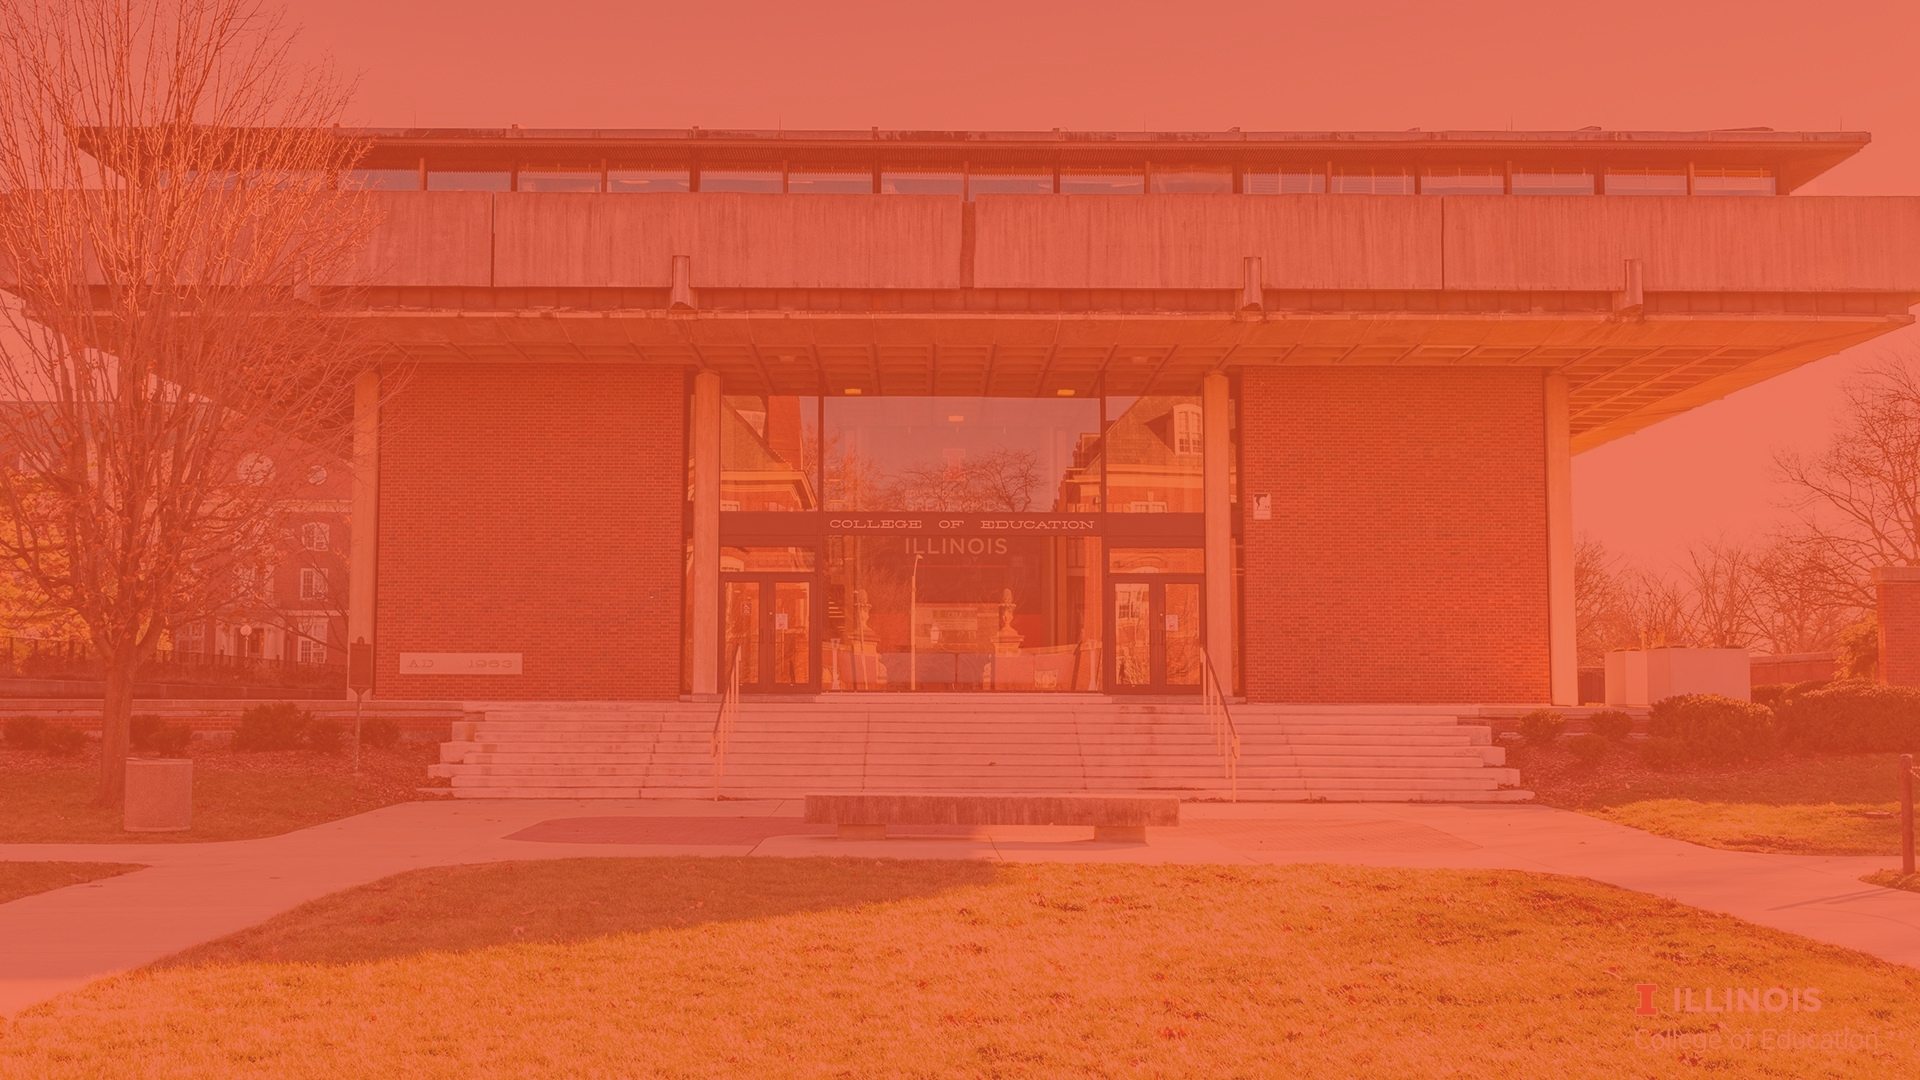
\includegraphics[width=\paperwidth, height=\paperheight]{imgs/uiuc.jpg}
    \end{textblock*} 
}{}

\begin{document}

\tikzstyle{vertex}=[circle,fill=black!25,minimum size=20pt,inner sep=0pt]
\tikzstyle{selected vertex} = [vertex, fill=orange!24]
\tikzstyle{edge} = [draw,thick,-]
\tikzstyle{weight} = [font=\small]
\tikzstyle{selected edge} = [draw,line width=5pt,-,blue!50]
\tikzstyle{ignored edge} = [draw,line width=5pt,-,black!20]


\frame{\titlepage}

\section{Objectives}
\begin{frame}
    \frametitle{Objectives}
    \begin{enumerate}
        \item Undstand the utility of big-O notation
        \item Compare ArrayList and LinkedList on the basis of big-O notation
        \item Understand the distinction between stacks and queues.
        \item Use the Queue interface and Stack and their common methods in Java. 
        \item Use a stack to build an RPN calculator.
        \item Use a queue to simulate round robin process scheduling.
    \end{enumerate}
\end{frame}

\section{big-O Notation}

\begin{frame}
    \frametitle{Algorithmic Complexity}
    \begin{enumerate}
        \item \textbf{Definition:} A way of defining the number of ``operations'' and ``amount of memory'' an algorithm (method) will take depending on the size of the input ($N$).
            \pause
        \item We consider two modes of complexity:
        \begin{itemize}
            \item \textbf{Time Complexity:} The number of operations we can expect an operation to take, in the worst case.
            \item \textbf{Space Complexity:} The amount of memory we can expect an operation to take, in the worst case.
        \end{itemize}
        \pause
        \item Today we will focus on time complexity.
        \pause
        \item Denoted as $O(\text{input space})$ to represent the upper bound (i.e., the worst case).
    \end{enumerate}
\end{frame}

\begin{frame}[fragile]
    \frametitle{Analyzing Algorithms}
    \centering
    \begin{minipage}{0.45\textwidth}
        \begin{lstlisting}[frame=trBL, basicstyle=\tiny]
public void printList(Integer item){
    System.out.println(item);
}
        \end{lstlisting}
    \end{minipage}
    \hfill
    \begin{minipage}{0.49\textwidth}
        \begin{lstlisting}[frame=trBL, basicstyle=\tiny]
public void printList(List<Integer> lst){
    for(int i = 0; i < lst.size(); i++){
        System.out.println(lst.get(i));
    }
}
        \end{lstlisting}
    \end{minipage}
    \begin{lstlisting}[frame=trBL, basicstyle=\tiny]
public void multiplyAndPrint(Integer item1, Integer item2){
    int result = item1 * item2;
    System.out.println(result);
}
    \end{lstlisting}
    \vfill
    {\large What is the maximum number of operations each method will perform? What is the minimum?}
\end{frame}

\begin{frame}[fragile]
    \frametitle{An example of constant time}
    \begin{lstlisting}[frame=trBL, basicstyle=\tiny]
public void multiplyAndPrint(Integer item1, Integer item2){
    int result = item1 * item2;
    System.out.println(result);
}
    \end{lstlisting}
    \begin{lstlisting}[frame=trBL, basicstyle=\tiny]
public void pow(Integer item1, Integer item2){
    int result = item1 * item2;
    System.out.println(result);
}
    \end{lstlisting}
    \begin{lstlisting}[frame=trBL, basicstyle=\tiny]
public void multiplyAndPrint(Integer item1, Integer item2){
    int result = item1 * item2;
    System.out.println(result);
}
    \end{lstlisting}
    \vfill
    {\large All of the above are treated as $O(1)$ since they don't increase with input size.}
\end{frame}

\begin{frame}[fragile]
    \frametitle{Analyzing Algorithms}
    \centering
    \begin{minipage}{0.7\textwidth}
    \centering
    \begin{lstlisting}[frame=trBL, basicstyle=\tiny]
public void printList(List<Integer> lst){
    for(int i = 0; i < lst.size(); i++){
        System.out.println(lst.get(i));
    }
}
    \end{lstlisting}
    \begin{lstlisting}[frame=trBL, basicstyle=\tiny]
public void printList(List<Integer> lst){
    for(int i = 0; i < lst.size(); i++){
        for(int j = 0; j < lst.size(); j++){
            System.out.println(lst.get(i) * lst.get(j));
        }
    }
}
    \end{lstlisting}
    \end{minipage}
    \hfill
    \begin{minipage}{0.29\textwidth}
    \hfill
    \end{minipage}
    \vfill
    {\large If one for loop (the first one) is $O(N)$, what is a nested for loop (the second one)?}
    \vfill
\end{frame}

\begin{frame}[fragile]
    \frametitle{Analyzing Algorithms}
    \centering
    \begin{minipage}{0.7\textwidth}
    \centering
    \begin{lstlisting}[frame=trBL, basicstyle=\tiny]
public void printList(List<Integer> lst){
    for(int i = 0; i < lst.size(); i++){
        System.out.println(lst.get(i));
    }
    for(int i = 0; i < lst.size(); i++){
        System.out.println(lst.get(i));
    }
}
    \end{lstlisting}
    \end{minipage}
    \hfill
    \begin{minipage}{0.29\textwidth}
    \hfill
    \end{minipage}
    \vfill
    {\large So is two for loops, unnested, $O(2N)$?}. 
    \vfill
\end{frame}


\begin{frame}[fragile]
    \frametitle{Examples}
	\begin{figure}
    \resizebox{\textheight}{!}{
    \begin{tikzpicture}[
        mystyle/.style={above, style = {font=\large}}
        ]
        \begin{axis}[
            % grid = major,
            clip = true, ticks = none,
            width = 15cm, height = 10cm,
            enlargelimits = false,
            scale only axis = true,
            every axis plot/.append style = {very thick},
            axis line style = ultra thick,
            clip mode = individual,
            domain = 0:10,
            restrict y to domain=0:10,
            restrict x to domain=0:10,
            axis x line = left, axis y line = left,
            xmin = 0, xmax = 11,
            ymin = 0, ymax = 11,
            xlabel = {Elements}, ylabel = {Operations},
            label style = {font=\large\bfseries\sffamily},
            xlabel style = {at={(axis description cs:0.5,-0.05)}, anchor=south},
            ylabel style = {at={(axis description cs:0.05,0.5)}, anchor=south},
            ]
            \addplot[color=direct]       {1}                 node[mystyle]{\(\Omicron(1)\)};
            \addplot[color=logarithmic]  {log2 x}            node[mystyle]{\(\Omicron(\log n)\)};
            \addplot[color=linear]       {x}                 node[mystyle]{\(\Omicron(n)\)};
            \addplot[color=squared]      {x^2}               node[mystyle]{\(\Omicron(n^2)\)};
            \addplot[color=nlogarithmic] {x*(log2 x)}        node[mystyle]{\(\Omicron(n\log n)\)};
            \addplot[color=cubed]        {x^3}               node[mystyle]{\(\Omicron(n^3)\)};
            \addplot[color=factorial]    gnuplot{gamma(x+1)} node[mystyle, yshift=0.6cm]{\(\Omicron(n!)\)};
        \end{axis}
    \end{tikzpicture}}
	\end{figure}
\end{frame}

\section{big-O and Lists}
\begin{frame}[fragile]
    \frametitle{ArrayList vs LinkedList - Searching}
    \begin{lstlisting}[frame=trBL, basicstyle=\tiny]
public void search(ListNode<E> head, E data){
    ListNode<E> tmp = head;
    while(tmp != null && !tmp.data.equals(data)){
        tmp = tmp.next;
    }
    return tmp;
}
    \end{lstlisting}
    \vfill
    \begin{enumerate}
		\item \textbf{LinkedList:} O(N) since we have to traverse to find the item.
		\item \textbf{ArrayList:} O(N) since we also have to traverse the item.
	\end{enumerate}
\end{frame}

\begin{frame}
    \frametitle{ArrayList vs LinkedList - Getting Item at Index}
    \begin{enumerate}
		\item What is the complexity of getting an item at an arbitrary position in a LinkedList? And an ArrayList?
            \pause
		\begin{enumerate}
			\item \textbf{LinkedList:} O(N) since we have to traverse to find the item.
			\item \textbf{ArrayList:} O(1) since we can index.
		\end{enumerate}
            \pause
		\item What would the complexity be for getFront() or getEnd() be for a LinkedList? How would this depend on whether we are keeping track of the tail?
            \pause
		\begin{enumerate}
			\item \textbf{LinkedList wo/ tail:} $O(1)$ to get head and $O(N)$ to get last node.
			\item \textbf{LinkedList w/ tail:} $O(1)$ for each.
		\end{enumerate}
    \end{enumerate}
\end{frame}

\begin{frame}
    \frametitle{ArrayList vs LinkedList - Insertion/Removal}
    \begin{enumerate}
        \item Adding/removing in the front?
            \pause
        \begin{enumerate}
            \item \textbf{LinkedList:} We track the head so we can just add on to the front, O(1).
            \item \textbf{ArrayList:} Finding the position is O(1) and copy/shift is O(N).
        \end{enumerate}
            \pause
        \item Adding/removing in the middle?
            \pause
        \begin{enumerate}
            \item \textbf{LinkedList:} Finding the position(s) is O(N).
            \item \textbf{ArrayList:} Finding the position is fast (O(1)) buth copy/shift makes this O(N).
            \item So both are O(N).
        \end{enumerate}
            \pause
        \item Adding/removing to the end?
            \pause
        \begin{enumerate}
            \item \textbf{LinkedList (wo/tail):} O(N) since we have to search for the end.
            \item \textbf{LinkedList (w/tail):} O(1) for adding since we track the tail.
            \item \textbf{ArrayList:} Finding the position is O(1) and since it's at the end 
        \end{enumerate}
    \end{enumerate}
\end{frame}


\section{Stacks}
\begin{frame}
    \frametitle{Stacks}
    \begin{enumerate}
        \item Last in, First out (LIFO) data structure.
        \item \lstinline|Stack| is a class Java
        \item Uses the following operations:
        \begin{enumerate}
            \item \lstinline|push| to add to the top of the stack.
            \item \lstinline|pop| to remove the element at the top of the stack.
        \end{enumerate}
    \end{enumerate}
\end{frame}

\section{Pushing}
\begin{frame}[fragile]
    \begin{figure}[H]
        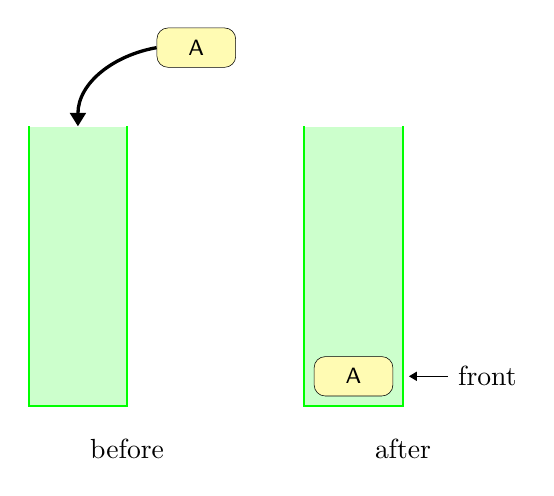
\begin{tikzpicture}
            \matrix[queue] (Q1) {
                |[fill=none, draw=none]| \\
                |[fill=none, draw=none]| \\
                |[fill=none, draw=none]| \\
                |[fill=none, draw=none]| \\
                |[fill=none, draw=none]| \\
            };
            \draw[green,thick,-] (Q1.north west) |-(Q1.south)-| (Q1.north east);
            %\draw[<-] ([xshift=.2cm]front.east) -- ++ (0:.5) node[right] {front};
            %\draw[<-] ([xshift=.2cm]rear.east) -- ++ (0:.5) node[right] {rear};
            \draw[<-,very thick] (Q1.north) to[out=90,in=190] ++ (1,1) node[right, queue element] (A) {A};
            \node[below=3mm of Q1.south east] {before};

            \scope[xshift=3.5cm] % queue after
            \matrix[queue] (Q1) {
                |[fill=none, draw=none]| \\
                |[fill=none, draw=none]| \\
                |[fill=none, draw=none]| \\
                |[fill=none, draw=none]| \\
            |(front)| A\\};
            \draw[green,thick,-] (Q1.north west) |-(Q1.south)-| (Q1.north east);
            \draw[<-] ([xshift=.2cm]front.east) -- ++ (0:.5) node[right] {front};
            %\draw[<-] ([xshift=.2cm]rear.east) -- ++ (0:.5) node[right] {rear};
            \node[below=3mm of Q1.south east] {after};
            \endscope
        \end{tikzpicture}
    \end{figure}
    \vfill
    \begin{lstlisting}[frame=trBL]
Stack<Integer> nums = new Stack<>();
nums.push("A")


    \end{lstlisting}
\end{frame}

\begin{frame}[fragile]
    \begin{figure}[H]
        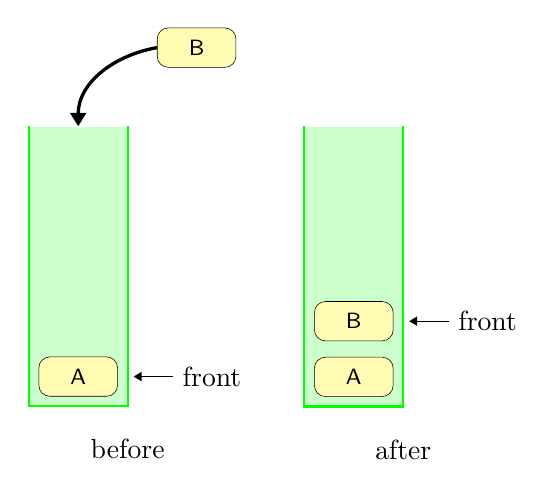
\begin{tikzpicture}
            \matrix[queue] (Q1) {
                |[fill=none, draw=none]| \\
                |[fill=none, draw=none]| \\
                |[fill=none, draw=none]| \\
                |[fill=none, draw=none]| \\
            |(front)| A\\};
            \draw[green,thick,-] (Q1.north west) |-(Q1.south)-| (Q1.north east);
            \draw[<-] ([xshift=.2cm]front.east) -- ++ (0:.5) node[right] {front};
            %\draw[<-] ([xshift=.2cm]rear.east) -- ++ (0:.5) node[right] {rear};
            \draw[<-,very thick] (Q1.north) to[out=90,in=190] ++ (1,1) node[right, queue element] (B) {B};
            \node[below=3mm of Q1.south east] {before};

            \scope[xshift=3.5cm] % queue after
            \matrix[queue] (Q1) {
                |[fill=none, draw=none]| \\
                |[fill=none, draw=none]| \\
                |[fill=none, draw=none]| \\
                |(front)| B \\
            |(rear)| A\\};
            \draw[green,thick,-] (Q1.north west) |-(Q1.south)-| (Q1.north east);
            \draw[<-] ([xshift=.2cm]front.east) -- ++ (0:.5) node[right] {front};
            %\draw[<-] ([xshift=.2cm]rear.east) -- ++ (0:.5) node[right] {rear};
            \node[below=3mm of Q1.south east] {after};
            \endscope
        \end{tikzpicture}
    \end{figure}
    \vfill
    \begin{lstlisting}[frame=trBL]
Stack<Integer> nums = new Stack<>();
nums.push("A")
nums.push("B")

    \end{lstlisting}
\end{frame}

\begin{frame}[fragile]
    \begin{figure}[H]
        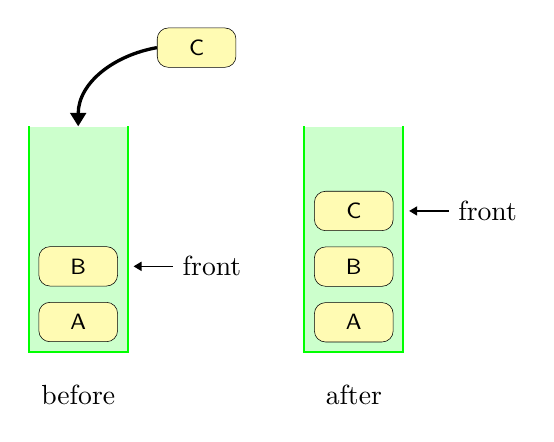
\begin{tikzpicture}
            \matrix[queue] (Q1) {
                |[fill=none, draw=none]| \\
                |[fill=none, draw=none]| \\
                |(front)| B\\
            |(rear)| A\\};
            \draw[green,thick,-] (Q1.north west) |-(Q1.south)-| (Q1.north east);
            \draw[<-] ([xshift=.2cm]front.east) -- ++ (0:.5) node[right] {front};
            %\draw[<-] ([xshift=.2cm]rear.east) -- ++ (0:.5) node[right] {rear};
            \draw[<-,very thick] (Q1.north) to[out=90,in=190] ++ (1,1) node[right, queue element] (C) {C};
            \node[below=3mm of Q1.south] {before};

            \scope[xshift=3.5cm] % queue after
            \matrix[queue] (Q1) {
                |[fill=none, draw=none]| \\
                |(front)|C\\
                B\\
            |(rear)| A\\};
            \draw[green,thick,-] (Q1.north west) |-(Q1.south)-| (Q1.north east);
            \draw[<-] ([xshift=.2cm]front.east) -- ++ (0:.5) node[right] {front};
            %\draw[<-] ([xshift=.2cm]rear.east) -- ++ (0:.5) node[right] {rear};
            \node[below=3mm of Q1.south] {after};
            \endscope
        \end{tikzpicture}
    \end{figure}
    \vfill
    \begin{lstlisting}[frame=trBL]
Stack<Integer> nums = new Stack<>();
nums.push("A")
nums.push("B")
nums.push("C")

    \end{lstlisting}
\end{frame}

\begin{frame}[fragile]
    \begin{figure}[H]
        \begin{tikzpicture}
            \matrix[queue] (Q1) {
                |[fill=none, draw=none]| \\
                |(front)| C\\
                B\\
            |(rear)| A\\};
            \draw[green,thick,-] (Q1.north west) |-(Q1.south)-| (Q1.north east);
            \draw[<-] ([xshift=.2cm]front.east) -- ++ (0:.5) node[right] {front};
            %\draw[<-] ([xshift=.2cm]rear.east) -- ++ (0:.5) node[right] {rear};
            \draw[<-,very thick] (Q1.north) to[out=90,in=190] ++ (1,1) node[right, queue element] (D) {D};
            \node[below=3mm of Q1.south east] {before};

            \scope[xshift=3.5cm] % queue after
            \matrix[queue] (Q1) {
                |(front)| D \\
                C\\
                B\\
            |(rear)| A\\};
            \draw[green,thick,-] (Q1.north west) |-(Q1.soutem \lstinline|dequeue|: to remove the element at the front of the queue.th)-| (Q1.north east);
            \draw[<-] ([xshift=.2cm]front.east) -- ++ (0:.5) node[right] {front};
            %\draw[<-] ([xshift=.2cm]rear.east) -- ++ (0:.5) node[right] {rear};
            \node[below=3mm of Q1.south east] {after};
            \endscope
        \end{tikzpicture}
    \end{figure}
    \vfill
    \begin{lstlisting}[frame=trBL]
Stack<Integer> nums = new Stack<>();
nums.push("A")
nums.push("B")
nums.push("C")
nums.push("D")
    \end{lstlisting}
\end{frame}

\section{Popping}
\begin{frame}[fragile]
    \begin{figure}[H]
        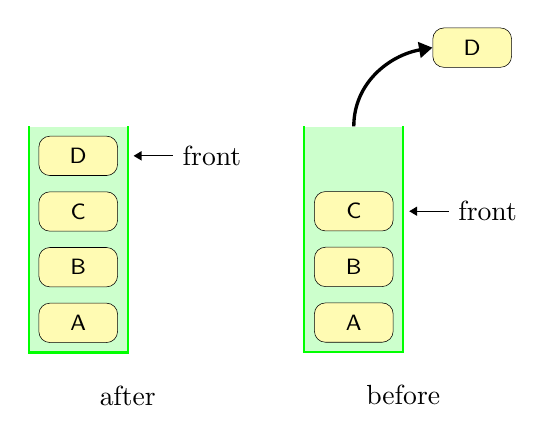
\begin{tikzpicture}
            \matrix[queue] (Q1) {
                |(front)| D \\
                C\\
                B\\
            |(rear)| A\\};
            \draw[green,thick,-] (Q1.north west) |-(Q1.south)-| (Q1.north east);
            \draw[<-] ([xshift=.2cm]front.east) -- ++ (0:.5) node[right] {front};
            %\draw[<-] ([xshift=.2cm]rear.east) -- ++ (0:.5) node[right] {rear};
            \node[below=3mm of Q1.south east] {after};
            \scope[xshift=3.5cm] % queue after
            \matrix[queue] (Q1) {
                |[fill=none, draw=none]| \\
                |(front)| C\\
                B\\
            |(rear)| A\\};
            \draw[green,thick,-] (Q1.north west) |-(Q1.south)-| (Q1.north east);
            \draw[<-] ([xshift=.2cm]front.east) -- ++ (0:.5) node[right] {front};
            %\draw[<-] ([xshift=.2cm]rear.east) -- ++ (0:.5) node[right] {rear};
            \draw[->,very thick] (Q1.north) to[out=90,in=190] ++ (1,1) node[right, queue element] (D) {D};
            \node[below=3mm of Q1.south east] {before};
            \endscope
        \end{tikzpicture}
    \end{figure}
    \vfill
    \begin{lstlisting}[frame=trBL]
Stack<Integer> nums = new Stack<>();
nums.push("A")
nums.push("B")
nums.push("C")
nums.push("D")
nums.pop()
    \end{lstlisting}
\end{frame}

\begin{frame}[fragile]
    \frametitle{Q: Where is this used? A: Call Stacks}
    \begin{minipage}{0.54\textwidth}
    \begin{lstlisting}[frame=trBL, basicstyle=\tiny]
public class PowerClass {
   
   public static int mult(int times, int val){
      int product = 0;
      for(int i = 0; i < times; i++){
         product += val;
      }
      return product;
   }
   
   public static int pow(int num, int raise){
      int total = 1;
      for(int i = 0; i < raise; i ++){
         total = mult(total, num);
      }
      return total;
   }
   
   public static void main(String[] args) {
      pow(2, 5);
   }
}
    \end{lstlisting}
    \end{minipage}
	\hfill
    \begin{minipage}{0.44\textwidth}
        \begin{drawstack}
            \cell{main()}
        \end{drawstack}
    \end{minipage}
    \centering 
    Our program starts at main.
\end{frame}

\begin{frame}[fragile]
    \frametitle{Q: Where is this used? A: Call Stacks}
    \begin{minipage}{0.54\textwidth}
    \begin{lstlisting}[frame=trBL, basicstyle=\tiny]
public class PowerClass {
   
   public static int mult(int times, int val){
      int product = 0;
      for(int i = 0; i < times; i++){
         product += val;
      }
      return product;
   }
   
   public static int pow(int num, int raise){
      int total = 1;
      for(int i = 0; i < raise; i ++){
         total = mult(total, num);
      }
      return total;
   }
   
   public static void main(String[] args) {
      pow(2, 5);
   }
}
    \end{lstlisting}
    \end{minipage}
	\hfill
    \begin{minipage}{0.44\textwidth}
        \begin{drawstack}
            \cell{pow(2, 5)}
            \cell{main()}
        \end{drawstack}
    \end{minipage}
    \centering 
    Our program starts at the pow method is then called an placed on the call stack.
\end{frame}

\begin{frame}[fragile]
    \frametitle{Q: Where is this used? A: Call Stacks}
    \begin{minipage}{0.54\textwidth}
    \begin{lstlisting}[frame=trBL, basicstyle=\tiny]
public class PowerClass {
   
   public static int mult(int times, int val){
      int product = 0;
      for(int i = 0; i < times; i++){
         product += val;
      }
      return product;
   }
   
   public static int pow(int num, int raise){
      int total = 1;
      for(int i = 0; i < raise; i ++){
         total = mult(total, num);
      }
      return total;
   }
   
   public static void main(String[] args) {
      pow(2, 5);
   }
}
    \end{lstlisting}
    \end{minipage}
	\hfill
    \begin{minipage}{0.44\textwidth}
        \begin{drawstack}
            \cell{mult(1, 2)}
            \cell{pow(2, 5)}
            \cell{main()}
        \end{drawstack}
    \end{minipage}
    \centering 
    The pow method then calls the mutl method.
\end{frame}

\begin{frame}[fragile]
    \frametitle{Q: Where is this used? A: Call Stacks}
    \begin{minipage}{0.54\textwidth}
    \begin{lstlisting}[frame=trBL, basicstyle=\tiny]
public class PowerClass {
   
   public static int mult(int times, int val){
      int product = 0;
      for(int i = 0; i < times; i++){
         product += val;
      }
      return product;
   }
   
   public static int pow(int num, int raise){
      int total = 1;
      for(int i = 0; i < raise; i ++){
         total = mult(total, num);
      }
      return total;
   }
   
   public static void main(String[] args) {
      pow(2, 5);
   }
}
    \end{lstlisting}
    \end{minipage}
	\hfill
    \begin{minipage}{0.44\textwidth}
        \begin{drawstack}
            \cell{pow(2, 5)}
            \cell{main()}
        \end{drawstack}
    \end{minipage}
    \centering 
    Once the call to mult is completed it is ``popped'' off of the stack and we return to where we left off in pow.
\end{frame}

\begin{frame}[fragile]
    \frametitle{Q: Where is this used? A: Call Stacks}
    \begin{minipage}{0.54\textwidth}
    \begin{lstlisting}[frame=trBL, basicstyle=\tiny]
public class PowerClass {
   
   public static int mult(int times, int val){
      int product = 0;
      for(int i = 0; i < times; i++){
         product += val;
      }
      return product;
   }
   
   public static int pow(int num, int raise){
      int total = 1;
      for(int i = 0; i < raise; i ++){
         total = mult(total, num);
      }
      return total;
   }
   
   public static void main(String[] args) {
      pow(2, 5);
   }
}
    \end{lstlisting}
    \end{minipage}
	\hfill
    \begin{minipage}{0.44\textwidth}
        \begin{drawstack}
            \cell{mult(2, 2)}
            \cell{pow(2, 5)}
            \cell{main()}
        \end{drawstack}
    \end{minipage}
    \centering 
    We then call the mult method again.
\end{frame}

\begin{frame}[fragile]
    \frametitle{Q: Where is this used? A: Call Stacks}
    \begin{minipage}{0.54\textwidth}
    \begin{lstlisting}[frame=trBL, basicstyle=\tiny]
public class PowerClass {
   
   public static int mult(int times, int val){
      int product = 0;
      for(int i = 0; i < times; i++){
         product += val;
      }
      return product;
   }
   
   public static int pow(int num, int raise){
      int total = 1;
      for(int i = 0; i < raise; i ++){
         total = mult(total, num);
      }
      return total;
   }
   
   public static void main(String[] args) {
      pow(2, 5);
   }
}
    \end{lstlisting}
    \end{minipage}
	\hfill
    \begin{minipage}{0.44\textwidth}
        \begin{drawstack}
            \cell{main()}
        \end{drawstack}
    \end{minipage}
    \centering 
    We continue this until pow is complete and then pop it off the stack.
\end{frame}

\begin{frame}[fragile]
    \frametitle{Q: Where is this used? A: Call Stacks}
    \begin{minipage}{0.54\textwidth}
    \begin{lstlisting}[frame=trBL, basicstyle=\tiny]
public class PowerClass {
   
   public static int mult(int times, int val){
      int product = 0;
      for(int i = 0; i < times; i++){
         product += val;
      }
      return product;
   }
   
   public static int pow(int num, int raise){
      int total = 1;
      for(int i = 0; i < raise; i ++){
         total = mult(total, num);
      }
      return total;
   }
   
   public static void main(String[] args) {
      pow(2, 5);
   }
}
    \end{lstlisting}
    \end{minipage}
	\hfill
    \begin{minipage}{0.44\textwidth}
        \begin{drawstack}
        \end{drawstack}
    \end{minipage}
    \centering 
    main has finished so that is popped as well and the program terminates.
\end{frame}




\begin{frame}
    \frametitle{Worksheet: Stack Practice}
    \centering
    \vfill
    Off to work on the worksheet to play with stacks.
    \vfill
\end{frame}


\begin{frame}
    \frametitle{RPN Calculator}
    Look at each element in the list and, at each stage:
    \begin{enumerate}
        \item If an element is an operation (i.e., +/-):
            \begin{enumerate}
                \item Pop two numbers from the stack
                \item Perform the operation
                \item Push the result onto the stack
            \end{enumerate}
        \item Otherwise, it must be a string representation of a number so:
            \begin{enumerate}
                \item Convert it to an `Integer`
                \item Push it to the stack
            \end{enumerate}
    \end{enumerate}
\end{frame}

\begin{frame}
    \frametitle{Worksheet: RPN Calculator}
    \centering
    \vfill
    Off to work on the worksheet to implement the RPN calculator
    \vfill
\end{frame}

\section{Queues}
\begin{frame}
    \begin{enumerate}
        \item First in, First out (FIFO) data structure.
        \item \lstinline|Queue| is an interface in Java.
        \item Uses the following operations:
        \begin{enumerate}
            \item \lstinline|enqueue|: to add to the end of a queue.
            \item \lstinline|dequeue|: to remove the element at the front of the queue.
        \end{enumerate}
    \end{enumerate}
\end{frame}

\section{Enqueueing}
\begin{frame}[fragile]
    \begin{figure}[H]
        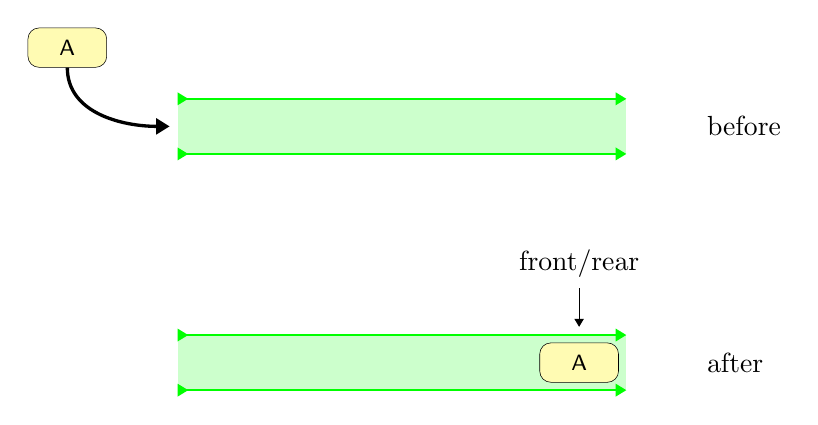
\begin{tikzpicture}
            \fill[green!20] (5.1,.35) rectangle (-.6,-.35);
            \draw[green,thick,>->] (-.6,.35) -- (5.1,.35);
            \draw[green,thick,>->] (-.6,-.35) -- (5.1,-.35);
            \path (6,0) node[right] {before};
            \node[queue element] (A) at (-2,1) {A};
            \draw[->,very thick] (A.south) to[out=-90,in=180] (-.7,0);

            \scope[yshift=-3cm] % queue after
            \fill[green!20] (5.1,.35) rectangle (-.6,-.35);
            \draw[green,thick,>->] (-.6,.35) -- (5.1,.35);
            \draw[green,thick,>->] (-.6,-.35) -- (5.1,-.35);
            \foreach \i/\name in {0/A}
            \node[queue element] (\name) at (4.5 - 1.5*\i,0) {\name};
            \draw[<-] ([yshift=.2cm]A.north) -- ++ (0,.5) node[above] {front/rear};
            \path (6,0) node[right] {after};
            \endscope
        \end{tikzpicture}
    \end{figure}
    \vfill
    \begin{lstlisting}[frame=trBL]
Queue<Integer> nums = new ArrayDequeue<>();
nums.offer("A")
    \end{lstlisting}
\end{frame}
\begin{frame}[fragile]
    \begin{figure}[H]
        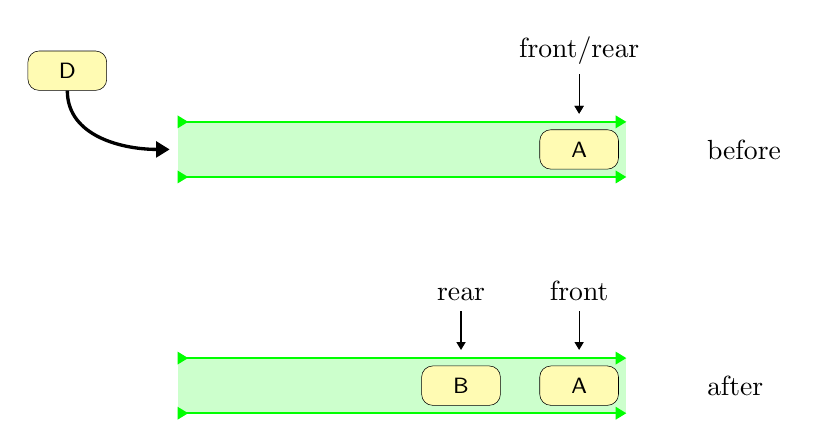
\begin{tikzpicture}
            \fill[green!20] (5.1,.35) rectangle (-.6,-.35);
            \draw[green,thick,>->] (-.6,.35) -- (5.1,.35);
            \draw[green,thick,>->] (-.6,-.35) -- (5.1,-.35);
            \foreach \i/\name in {0/A}
            \node[queue element] (\name) at (4.5 - 1.5*\i,0) {\name};
            \draw[<-] ([yshift=.2cm]A.north) -- ++ (0,.5) node[above] {front/rear};
            \draw[<-] ([yshift=.2cm]A.north) -- ++ (0,.5) node[above, xshift=-.5cm] {};
            \path (6,0) node[right] {before};
            \node[queue element] (D) at (-2,1) {D};
            \draw[->,very thick] (D.south) to[out=-90,in=180] (-.7,0);

            \scope[yshift=-3cm] % queue after
            \fill[green!20] (5.1,.35) rectangle (-.6,-.35);
            \draw[green,thick,>->] (-.6,.35) -- (5.1,.35);
            \draw[green,thick,>->] (-.6,-.35) -- (5.1,-.35);
            \foreach \i/\name in {0/A, 1/B}
            \node[queue element] (\name) at (4.5 - 1.5*\i,0) {\name};
            \draw[<-] ([yshift=.2cm]A.north) -- ++ (0,.5) node[above] {front};
            \draw[<-] ([yshift=.2cm]B.north) -- ++ (0,.5) node[above] {rear};
            \path (6,0) node[right] {after};
            \endscope
        \end{tikzpicture}
    \end{figure}
    \vfill
    \begin{lstlisting}[frame=trBL]
Queue<Integer> nums = new ArrayDequeue<>();
nums.offer("A")
nums.offer("B")


    \end{lstlisting}
\end{frame}
\begin{frame}[fragile]
    \begin{figure}[H]
        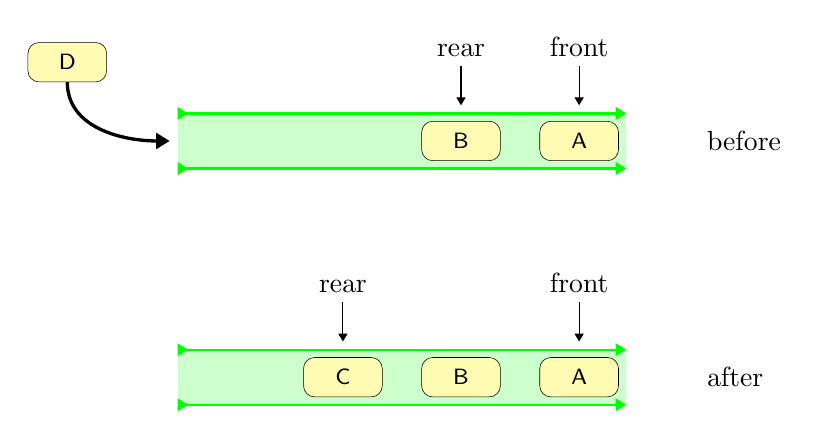
\begin{tikzpicture}
            \fill[green!20] (5.1,.35) rectangle (-.6,-.35);
            \draw[green,thick,>->] (-.6,.35) -- (5.1,.35);
            \draw[green,thick,>->] (-.6,-.35) -- (5.1,-.35);
            \foreach \i/\name in {0/A, 1/B}
            \node[queue element] (\name) at (4.5 - 1.5*\i,0) {\name};
            \draw[<-] ([yshift=.2cm]A.north) -- ++ (0,.5) node[above] {front};
            \draw[<-] ([yshift=.2cm]B.north) -- ++ (0,.5) node[above] {rear};
            \path (6,0) node[right] {before};
            \node[queue element] (D) at (-2,1) {D};
            \draw[->,very thick] (D.south) to[out=-90,in=180] (-.7,0);

            \scope[yshift=-3cm] % queue after
            \fill[green!20] (5.1,.35) rectangle (-.6,-.35);
            \draw[green,thick,>->] (-.6,.35) -- (5.1,.35);
            \draw[green,thick,>->] (-.6,-.35) -- (5.1,-.35);
            \foreach \i/\name in {0/A, 1/B, 2/C}
            \node[queue element] (\name) at (4.5 - 1.5*\i,0) {\name};
            \draw[<-] ([yshift=.2cm]A.north) -- ++ (0,.5) node[above] {front};
            \draw[<-] ([yshift=.2cm]C.north) -- ++ (0,.5) node[above] {rear};
            \path (6,0) node[right] {after};
            \endscope
        \end{tikzpicture}
    \end{figure}
    \vfill
    \begin{lstlisting}[frame=trBL]
Queue<Integer> nums = new ArrayDequeue<>();
nums.offer("A")
nums.offer("B")
nums.offer("C")

    \end{lstlisting}
\end{frame}
\begin{frame}[fragile]
    \begin{figure}[H]
        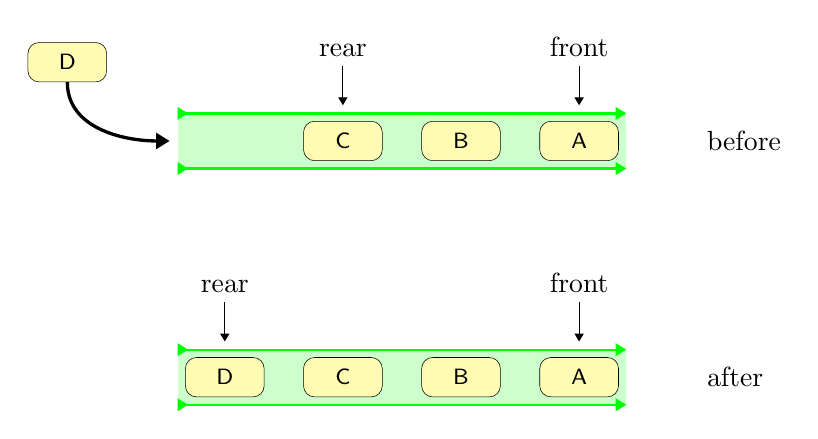
\begin{tikzpicture}
            \fill[green!20] (5.1,.35) rectangle (-.6,-.35);
            \draw[green,thick,>->] (-.6,.35) -- (5.1,.35);
            \draw[green,thick,>->] (-.6,-.35) -- (5.1,-.35);
            \foreach \i/\name in {0/A, 1/B, 2/C}
            \node[queue element] (\name) at (4.5 - 1.5*\i,0) {\name};
            \draw[<-] ([yshift=.2cm]A.north) -- ++ (0,.5) node[above] {front};
            \draw[<-] ([yshift=.2cm]C.north) -- ++ (0,.5) node[above] {rear};
            \path (6,0) node[right] {before};
            \node[queue element] (D) at (-2,1) {D};
            \draw[->,very thick] (D.south) to[out=-90,in=180] (-.7,0);

            \scope[yshift=-3cm] % queue after
            \fill[green!20] (5.1,.35) rectangle (-.6,-.35);
            \draw[green,thick,>->] (-.6,.35) -- (5.1,.35);
            \draw[green,thick,>->] (-.6,-.35) -- (5.1,-.35);
            \foreach \i/\name in {0/A, 1/B, 2/C, 3/D}
            \node[queue element] (\name) at (4.5 - 1.5*\i,0) {\name};
            \draw[<-] ([yshift=.2cm]A.north) -- ++ (0,.5) node[above] {front};
            \draw[<-] ([yshift=.2cm]D.north) -- ++ (0,.5) node[above] {rear};
            \path (6,0) node[right] {after};
            \endscope
        \end{tikzpicture}
    \end{figure}
    \vfill
    \begin{lstlisting}[frame=trBL]
Queue<Integer> nums = new ArrayDequeue<>();
nums.offer("A")
nums.offer("B")
nums.offer("C")
nums.offer("D")
    \end{lstlisting}
\end{frame}

\section{Dequeueing}
\begin{frame}[fragile]
    \begin{figure}[H]
        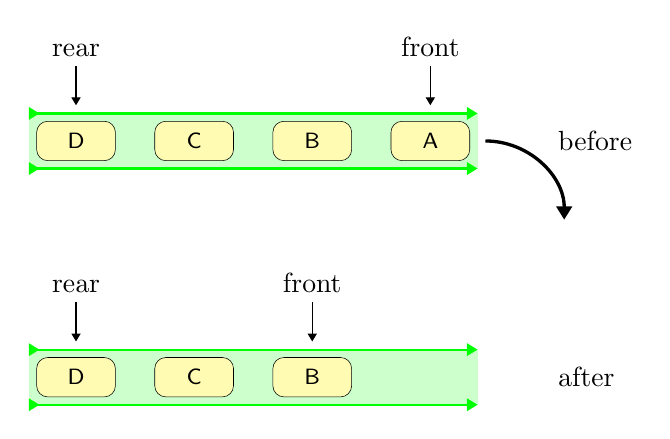
\begin{tikzpicture}
            \fill[green!20] (5.1,.35) rectangle (-.6,-.35);
            \draw[green,thick,>->] (-.6,.35) -- (5.1,.35);
            \draw[green,thick,>->] (-.6,-.35) -- (5.1,-.35);
            \foreach \i/\name in {0/D,1/C,2/B,3/A}
                \node[queue element] (\name) at (1.5*\i,0) {\name};
                \draw[<-] ([yshift=.2cm]A.north) -- ++ (0,.5) node[above] {front};
                \draw[<-] ([yshift=.2cm]D.north) -- ++ (0,.5) node[above] {rear};
                \draw[->,very thick] (5.2,0) to[out=0,in=90] ++ (1,-1);
                \path (6,0) node[right] {before};

                \scope[yshift=-3cm] % queue after
                \fill[green!20] (5.1,.35) rectangle (-.6,-.35);
                \draw[green,thick,>->] (-.6,.35) -- (5.1,.35);
                \draw[green,thick,>->] (-.6,-.35) -- (5.1,-.35);
                \foreach \i/\name in {0/D,1/C,2/B}
                \node[queue element] (\name) at (1.5*\i,0) {\name};
                \draw[<-] ([yshift=.2cm]B.north) -- ++ (0,.5) node[above] {front};
                \draw[<-] ([yshift=.2cm]D.north) -- ++ (0,.5) node[above] {rear};
                \path (6,0) node[right] {after};
                \endscope
            \end{tikzpicture}
    \end{figure}
    \begin{lstlisting}[frame=trBL]
Queue<Integer> nums = new ArrayDequeue<>();
nums.offer("A")
nums.offer("B")
nums.offer("C")
nums.offer("D")
nums.poll()
    \end{lstlisting}
\end{frame}

\begin{frame}
    \frametitle{Worksheet: Queue Practice}
    \centering
    \vfill
    Off to work on the worksheet to play with queues.
    \vfill
\end{frame}


\begin{frame}
    \frametitle{Process Scheduling}
    \begin{enumerate}
        \item Dequeue a process
        \item Check if the allowed processing time (quanta) is less than the time remaining to serve that proccess:
        \item If it is:
            \begin{enumerate}
                \item  reduce the proc's remaining time by that quanta
                \item  increment the total process time by the quanta
                \item  increment that proc's contex switch count
                \item  enqueue the process
                \item  Print a message indicating the name of the process and it's quanta
            \end{enumerate}
        \item  Otherwise:
            \begin{enumerate}
                \item  increment the total processing time by the time remaining for that process
                \item  print a message indicating the event name, the total time the process spent in the queue, and the number of time's it was switched out of context.
            \end{enumerate}
    \end{enumerate}
\end{frame}

\begin{frame}
    \frametitle{Worksheet: Round Robin Scheduler}
    \centering
    \vfill
    Off to work on the worksheet to implement a round robin simulator.
    \vfill
\end{frame}

\section{Card Games}
\begin{frame}
    \frametitle{Application: Card Game}
\end{frame}


\end{document}
